\subsection{Context}
\begin{frame}{Context}
\bi
\item Climate change is ongoing, want to reduce emissions
\item Reduce through increasing renewables
\ei

\pause
\centering
\vspace{.2in}
\alert{Emmissions of Electricity Generation}
\vspace{.2in}
\begin{columns}
\begin{column}{0.425\textwidth}
\centering
Canada
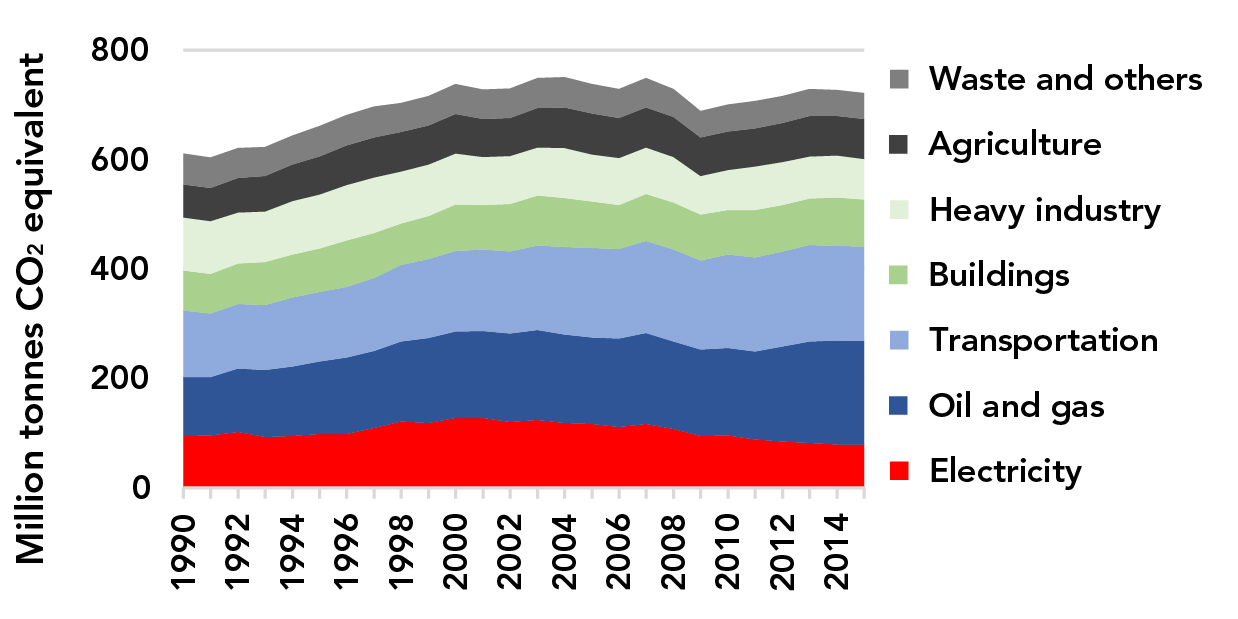
\includegraphics[height=1.15in]{ghg_emissions}
\end{column}
\begin{column}{0.425\textwidth}
\centering
Worldwide
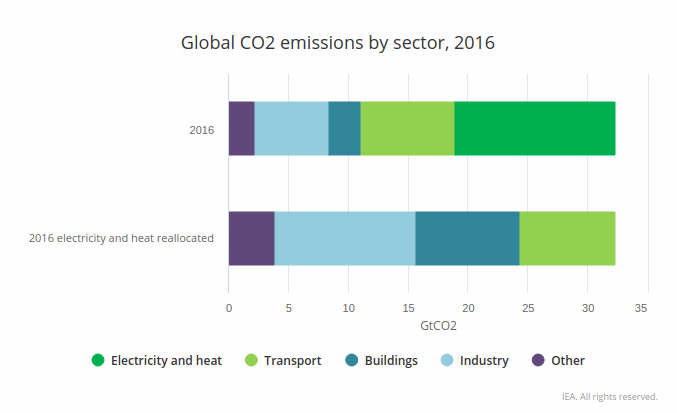
\includegraphics[height=1.15in]{ghg_emissions_worldwide}
\end{column}
\end{columns}
\end{frame}

\subsection{Power Systems Analysis}
\begin{frame}{Challenges}


\BBR{Bulk Power Systems (BPS)}
\bi
\item Composed of generation and high voltage transmission equipement.  
\item Goal to provide least cost electricity while maintaining reliability.
\ei
\EBR
\pause
\vspace{.3in}
\alert{Challenges}
\bi
\item Renewables [often] connect with bulk power system (BPS)
\item BPS must maintain system reliability
\item Renewables uncertain and not controllable
\ei
\end{frame}

\begin{frame}{Bulk Power Systems}

\only<1>{US split into 3 interconnected grids}
\only<2>{\sout{US split into 3 interconnected grids}}

\only<2>{\alert{North America split into 4 interconnected grids}}
\bi
\item Generators rotating synchronously with grid
\item Connection to every load
\ei



\end{frame}

\begin{frame}{North America Interconnections}
\centering
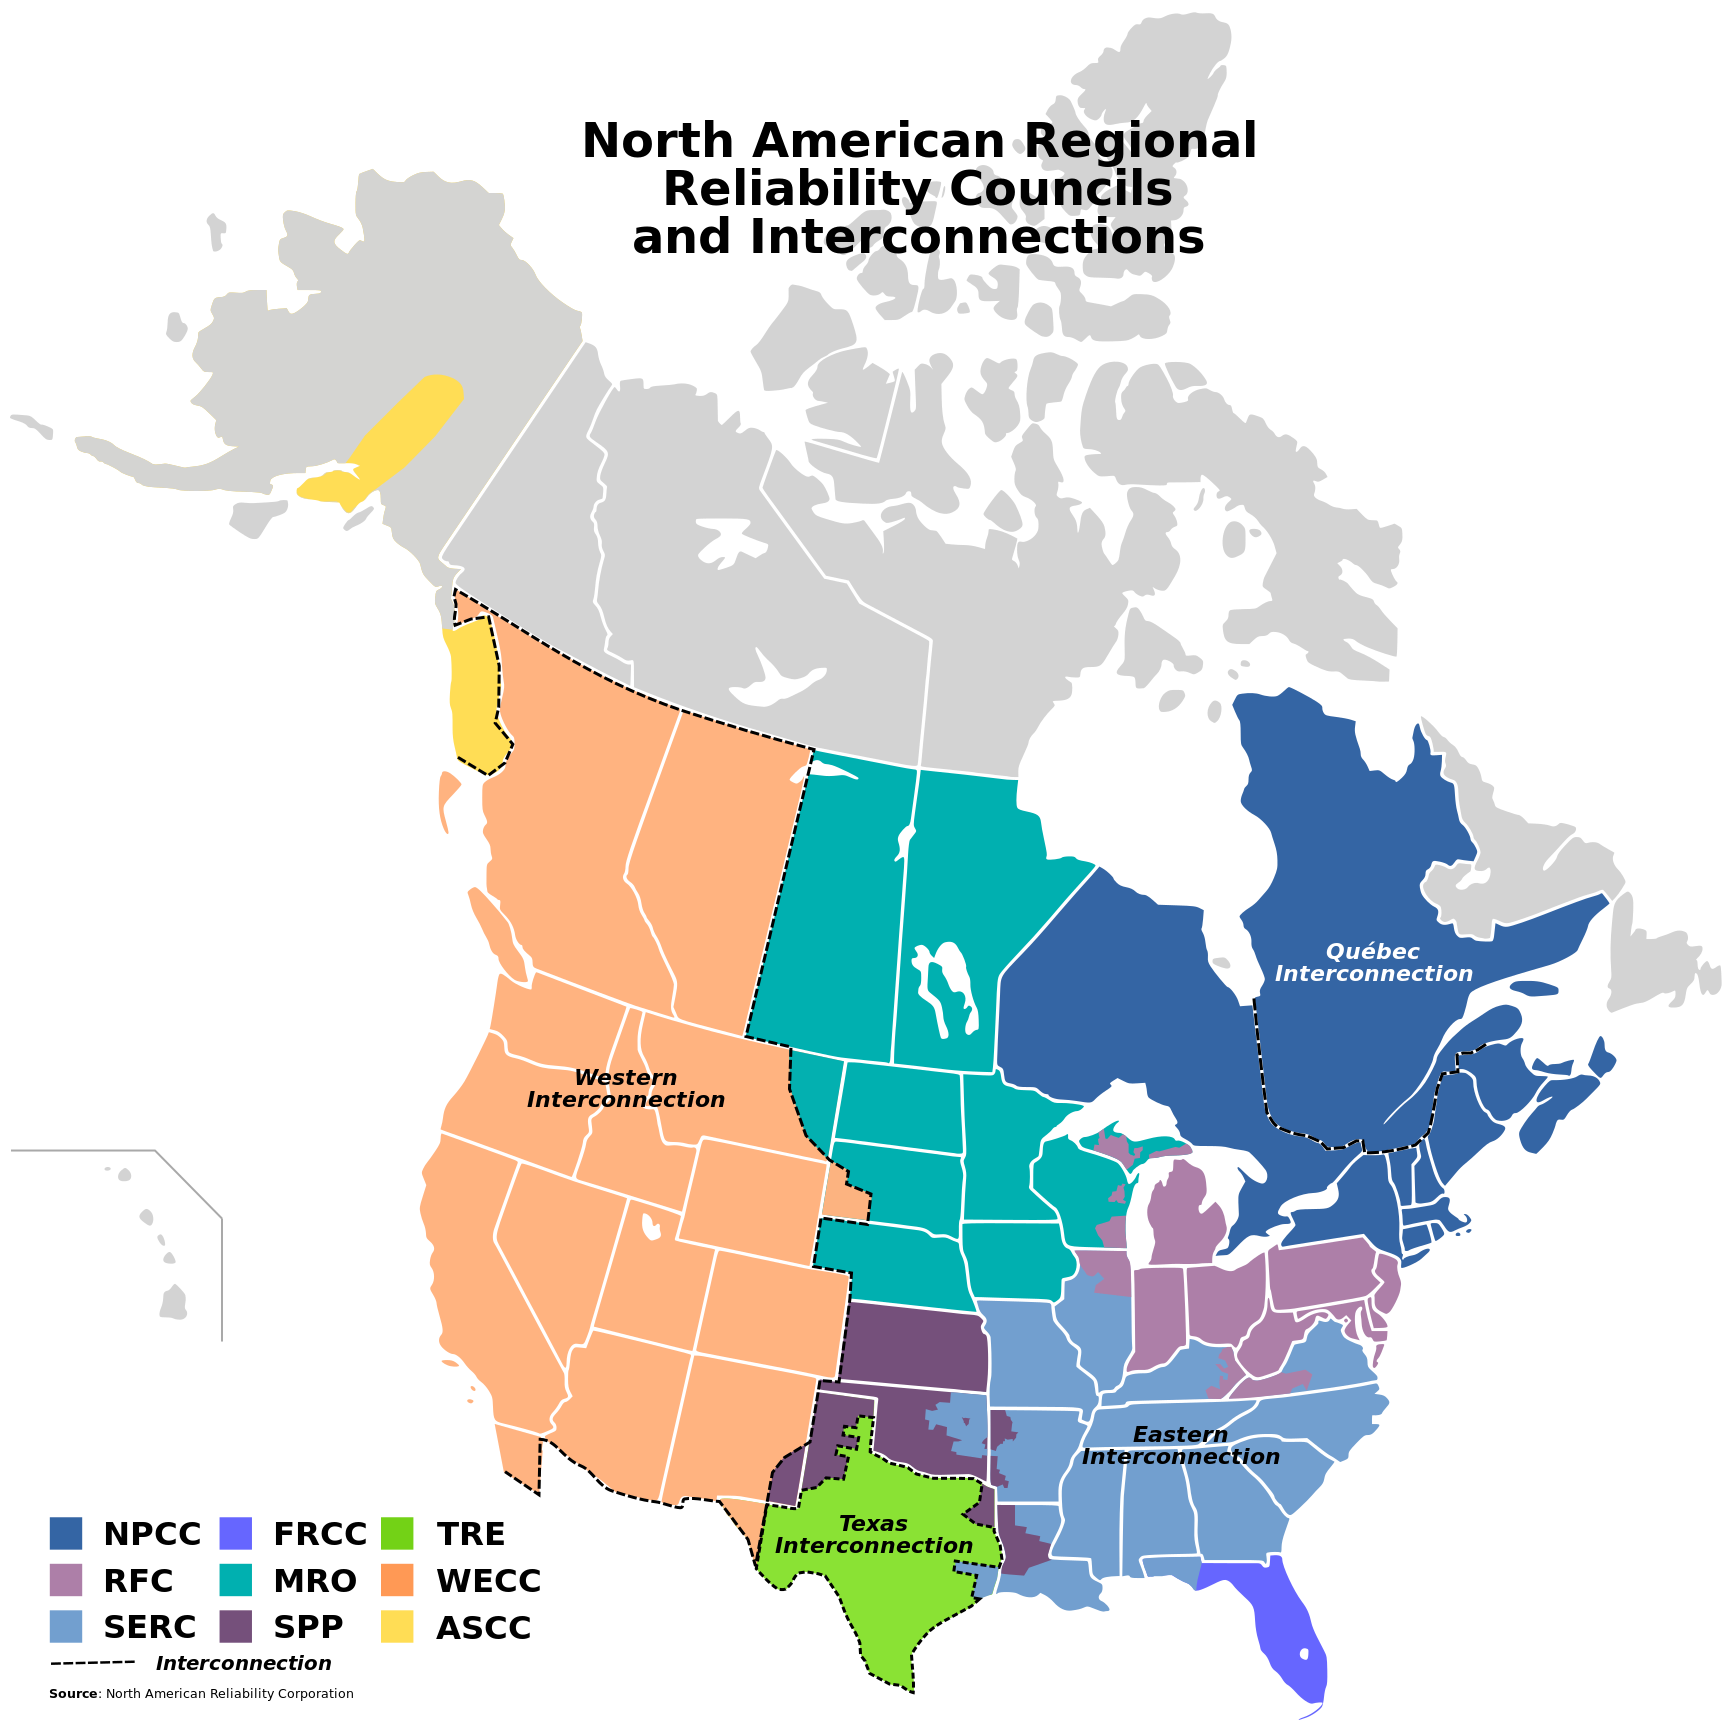
\includegraphics[height=3in]{interconnect.png}
\end{frame}

\begin{frame}{Bulk Power Systems}


Complex system requiring continuous supply demand balance

\bi
\item Transient stability, automatic generator control
\item Ancillary services market
\item \only<1>{ 5 minute real time market} \only<2>{\textcolor{red}{ 5 minute real time market}} 
\item 1-6 hour inter region market 
\item 24 hour day ahead market
\item Long term capacity markets
\ei
\end{frame}

\begin{frame}{Optimization in Power System}

\bi
\item Operational/Markets
	\bi
	\item Real time market / economic dispatch \only<2>{- \textcolor{red}{LP}}
	\item Day ahead market / unit commitment \only<2>{- \textcolor{red}{MIP}}
	\ei
\item Planning
	\bi
	\item Production cost model
		\only<2>{ \textcolor{red}{simulation - MIP}}
	\item Capacity expansion 
		\only<2>{\textcolor{red}{MIP / DFO}}
	\ei
\item Reliability
	\bi
	\item Power flow / optimal power flow \only<2>{- \textcolor{red}{NLP}}
	\item Dynamics / transient stability \only<2>{\textcolor{red}{simulation - NLP}}
	\ei
\ei


\only<2>{
\bi
	\item \textcolor{red}{LP} = Linear Program
	\item \textcolor{red}{MIP} = Mixed Integer Program
	\item \textcolor{red}{NLP} = Nonlinear Program
	\item \textcolor{red}{DFO} = Derivative Free Optimization
\ei}

\end{frame}

\begin{frame}{Power Flow}
Laws of physics, can't control branch flow

\alert{Control net injects}
\bi
\item Generators
\bi 
\item Ramping characterstics, limits
\ei
\item Demand Response
\item Storage (hydro, battery)
\ei

\pause

AC power flow - balanced 3 phase power system model 
\bi
\item Nonlinear, nonconvex equations
\item Difficult to solve
\item \alert{We use DC approximation (linear)}
\ei

%3 ways to solve
%\bi
%\item Local methods (i.e. Newton method, no optimality guarantees)
%\item Convex Relaxations (i.e. SDP [Lavaei and Low], Quadratic [Hijazi]) %put in footnote
%\bi
%\item Ability to distinguish numerical problems from systemic infeasibility
%\ei
%\item Approximations (i.e. DC power flow, linear approximation)
%\bi
%\item Reduction in computational complexity at cost to accuracy
%\item Extensions to capture voltage information and transmission losses
%\ei
%\ei
\end{frame}

\begin{frame}{ERCOT Snapshot}

\vspace{-4cm}
\hspace{-2cm}
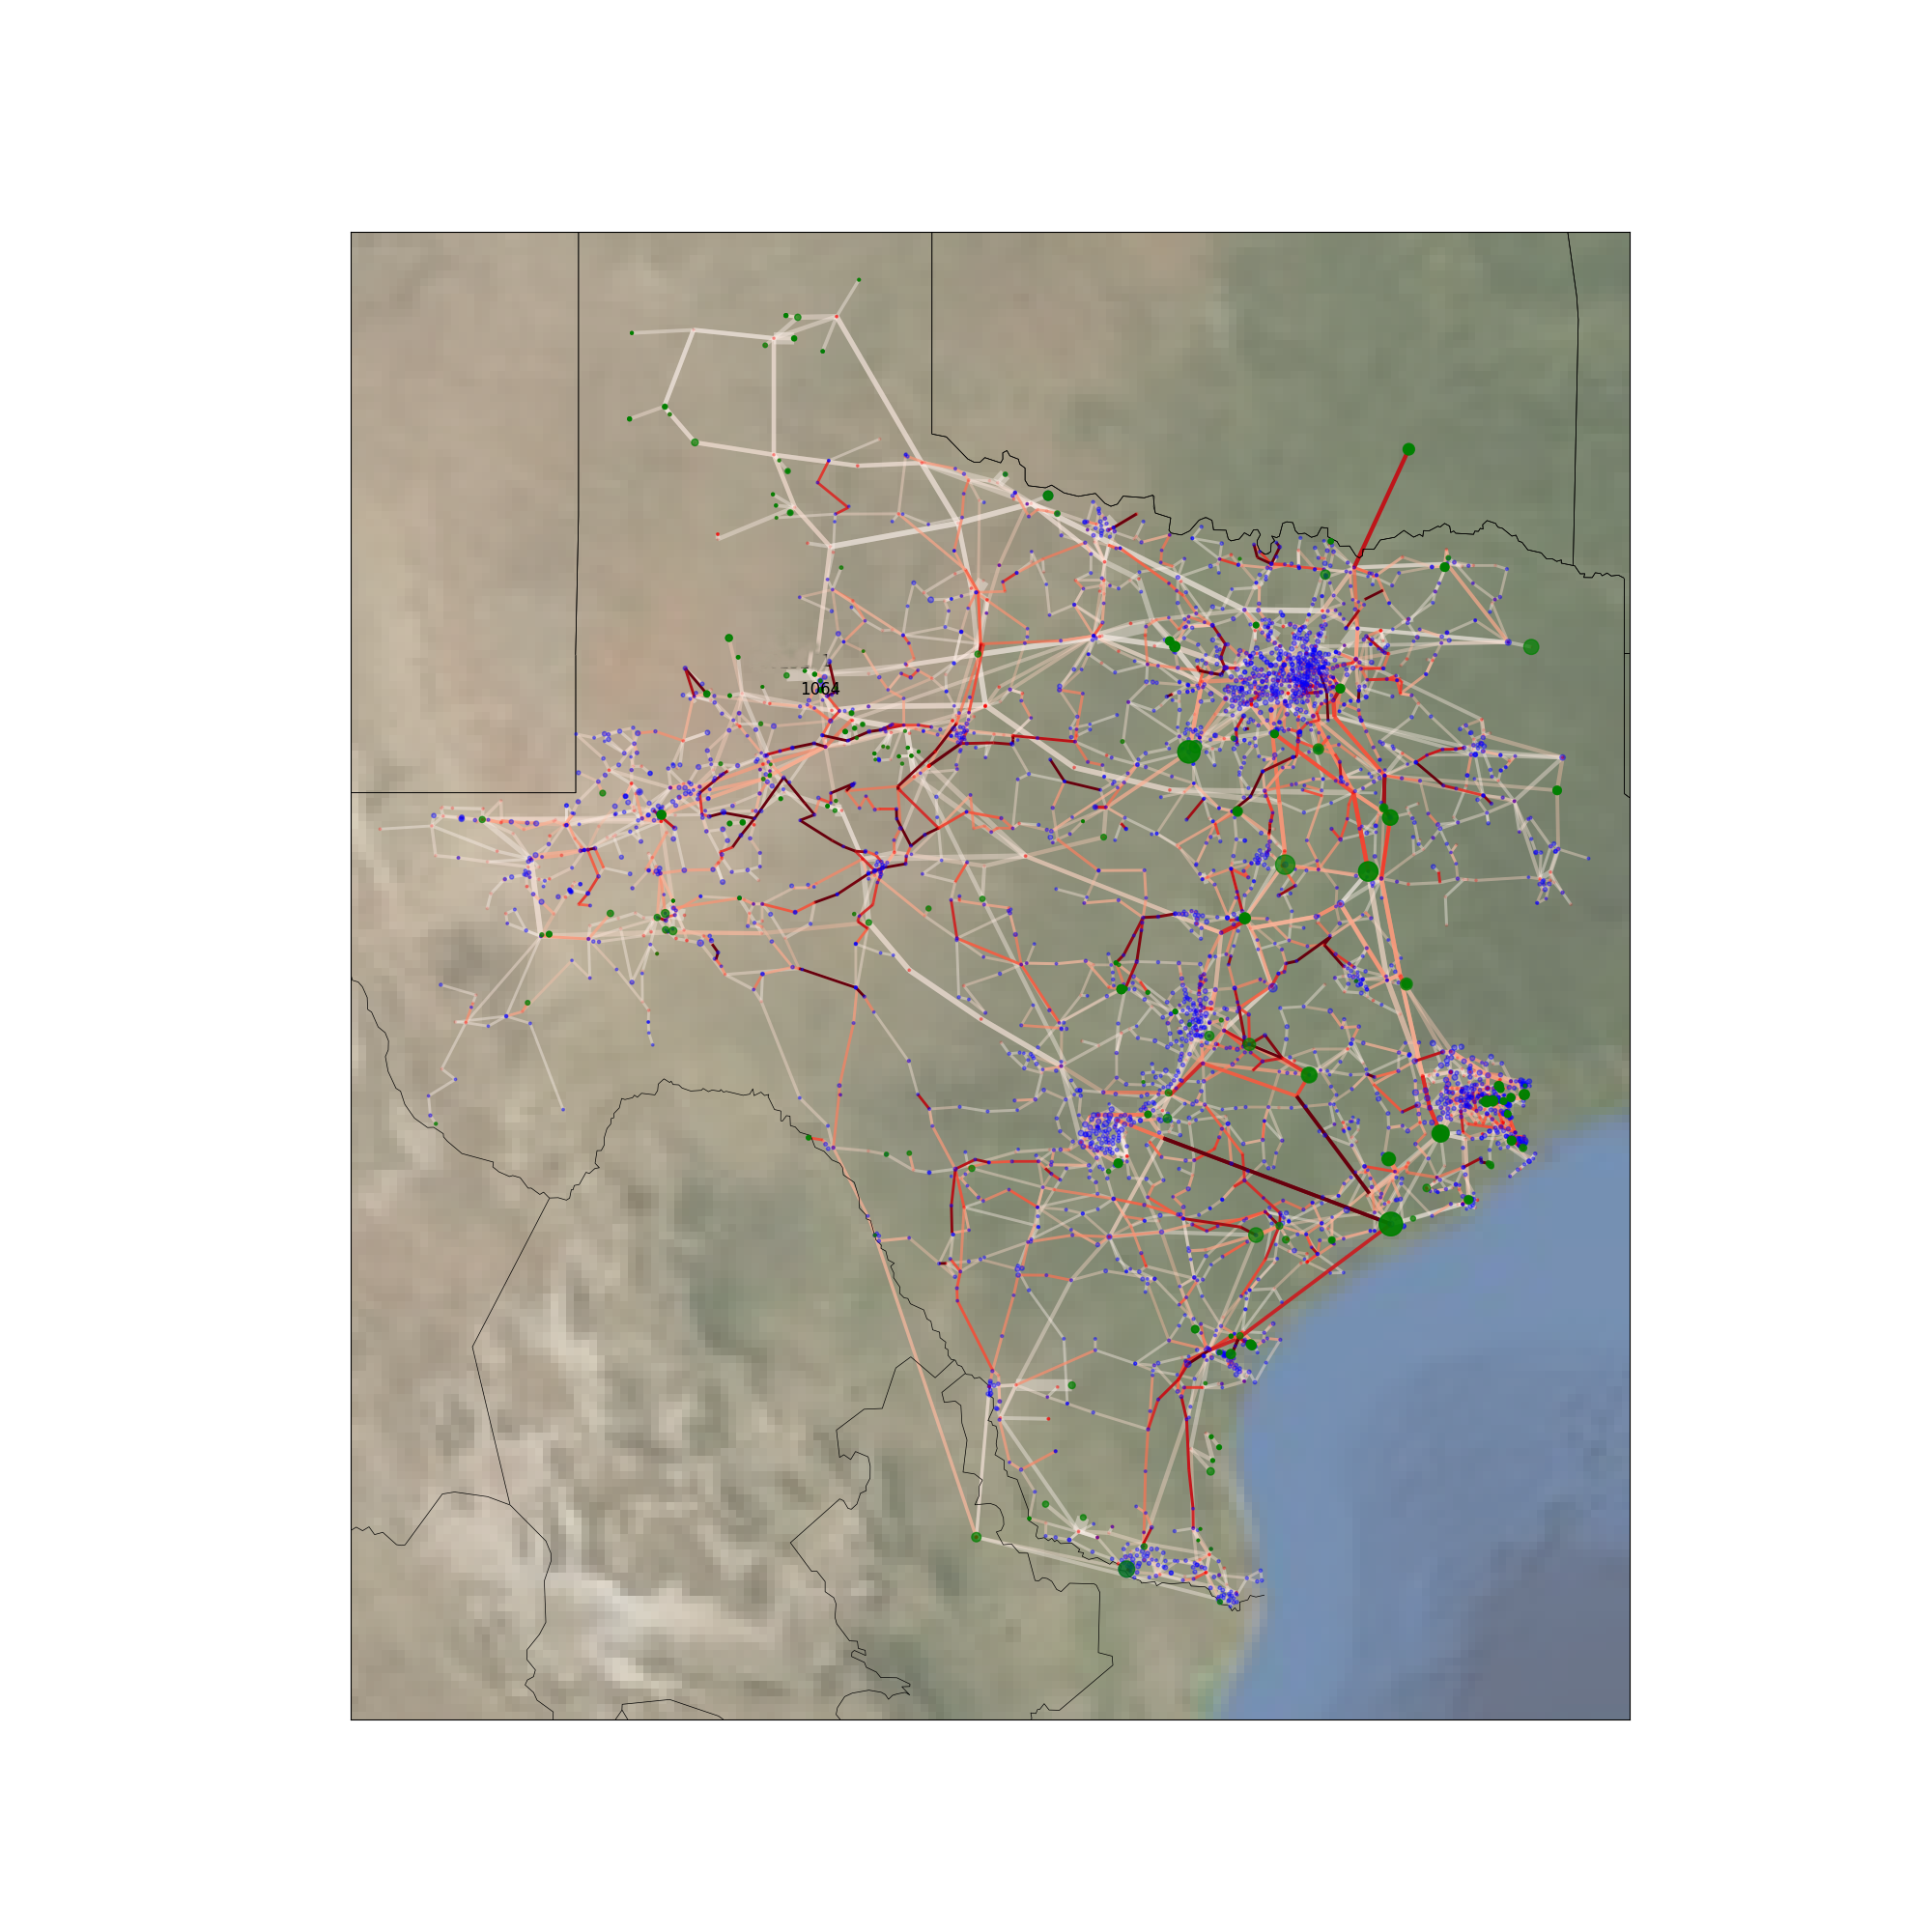
\includegraphics[height=6in,width=5in,trim={5cm 5cm 5cm 5cm},clip]{ercot_example.png}
\end{frame}

\subsection{Uncertainty}
\begin{frame}{Modern Complexity for Power Systems}

\alert{Uncertainty}

Asking more of our transmission grid, robust to uncertainty

\bi
\item Wind
\item Solar
\item Demand Response
\item Energy Storage
\item Electric Vehicles
\ei
\end{frame}

\bc{
\begin{frame}{Renewable Generation, Geographically Correlated}
\begin{center}
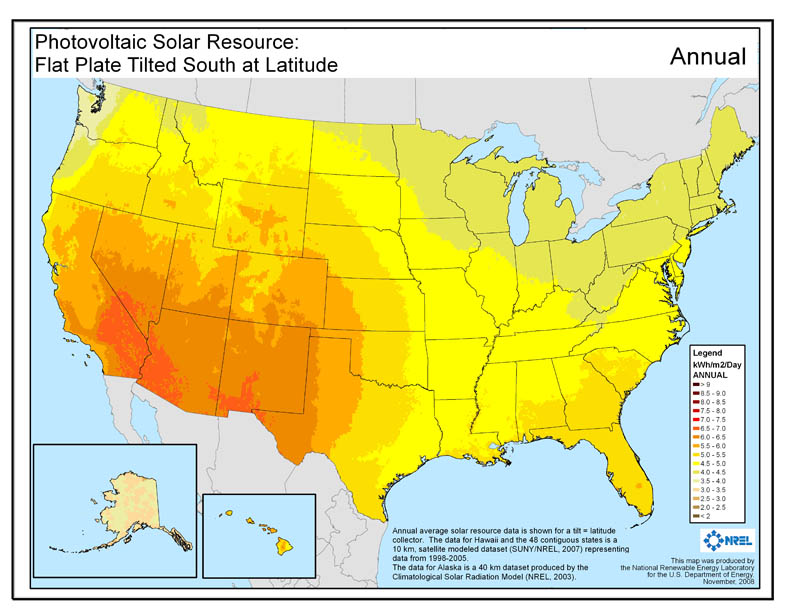
\includegraphics[height=1.4in]{solar-map} \hfill %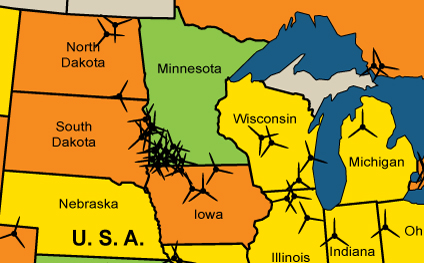
\includegraphics[height=1.4in]{windmap}
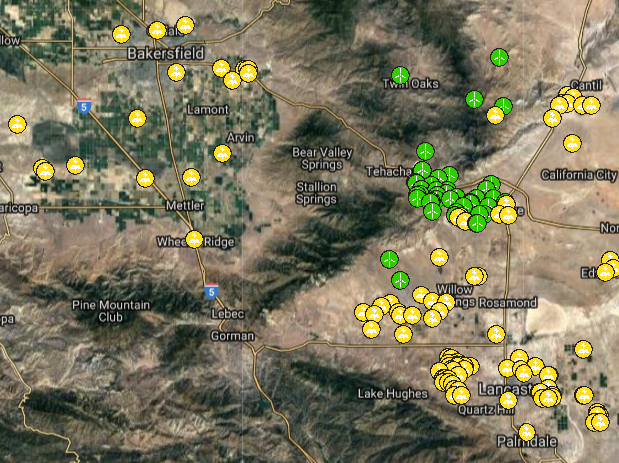
\includegraphics[height=1.4in]{renewables-correlated}
\end{center}
\end{frame}
}

\subsection{Reliability Problems}
\begin{frame}{Reliability Problems}
\alert{Power Interruptions}
\bi
\item \$79 billion economic loss (2001) 
\bi
\item \$247 billion electricity sales
\ei 
\item Hidden from system, distributed throughout economy
\item New technologies: renewables, EVs, etc. stressful on system
\ei
\pause
\alert{Cascading power failures}
\bi
\item Rare, but costly
\item Equillibrium balancing economics and reliability
\item Northeast blackout 2003
\bi
\item \$6 billion economic loss
\item Loss of life
\ei
\ei
\end{frame}